\documentclass{standalone}

\usepackage{graphics}
\usepackage[dvipsnames,svgnames]{xcolor}

\usepackage{tikz,pgf,pgfplots,circuitikz}
\pgfplotsset{compat=1.15}
\usetikzlibrary{intersections,arrows.meta,angles,calc,3d,decorations.pathmorphing}
\usepackage[compat=1.1.0]{tikz-feynhand}

\usepackage{amssymb,amsfonts,amsthm,mathtools}
\usepackage{physics,braket,bm}

\begin{document}
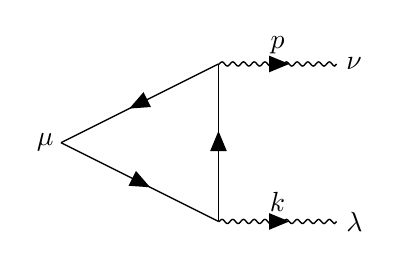
\begin{tikzpicture}
  \begin{feynhand}
    \vertex (p1) at (-1,0);
    \vertex (p2) at (1,1);    
    \vertex (p3) at (1,-1);
    \vertex (p4) at (2.5,1) [right] {$\nu$};    
    \vertex (p5) at (2.5,-1) [right] {$\lambda$};
    \propag [fermion] (p1) to (p3);
    \propag [fermion] (p3) to (p2);
    \propag [fermion] (p2) to (p1);
    \propag [charged boson] (p2) to [edge label=$p$] (p4);
    \propag [charged boson] (p3) to [edge label=$k$] (p5);
    \node at (-1.2,0) {$\mu$};
  \end{feynhand}
\end{tikzpicture}
\end{document}
